
\begin{figure}[H]
\centering
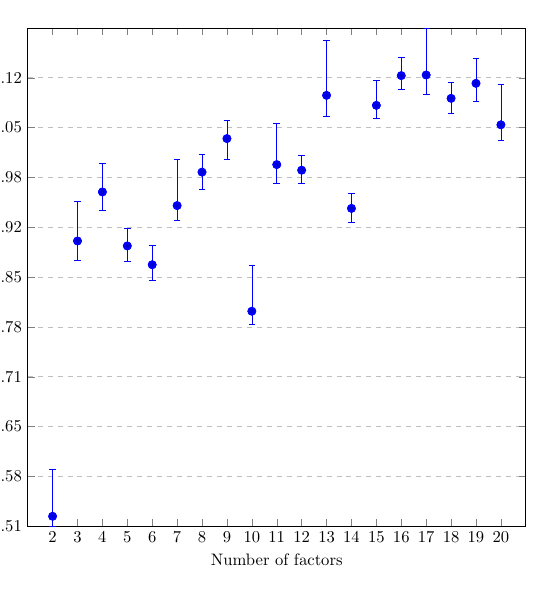
\begin{tikzpicture}[scale=0.6, trim axis left, trim axis right]
\begin{axis}[
    width=1\textwidth,
    height=1\textwidth,
    xlabel={Number of factors},
    ylabel={Time taken (s)},
    xmin=1.0, xmax=21.0,
    ymin=0.511378, ymax=1.185382,
    xticklabels={2, 3, 4, 5, 6, 7, 8, 9, 10, 11, 12, 13, 14, 15, 16, 17, 18, 19, 20},
    xtick={2, 3, 4, 5, 6, 7, 8, 9, 10, 11, 12, 13, 14, 15, 16, 17, 18, 19, 20},
    ytick={0.511378, 0.5787784, 0.6461788, 0.7135792, 0.7809796, 0.84838, 0.9157804, 0.9831808, 1.0505812, 1.1179816},
    ymajorgrids=true,
    grid style=dashed,
]

\addplot+[
    blue,
    very thick,
    forget plot,
    only marks
    ]
    plot[
    very thick,
    error bars/.cd,
    y dir=plus,
    y explicit
    ]
    table[x=x,y=y,y error expr=\thisrow{y-max}] {
    x    y    y-max
    11	1.00055786667	0.0557551333333
10	0.802164633333	0.0627623666667
13	1.09425033333	0.0750086666667
12	0.9929817	0.0201843
15	1.0807066	0.0343404
14	0.9413146	0.0206874
17	1.12181526667	0.0635667333333
16	1.12097466667	0.0249823333333
19	1.11051936667	0.0334966333333
18	1.09022053333	0.0217664666667
20	1.0544286	0.0550564
3	0.8972128	0.0534252
2	0.524697	0.063058
5	0.890506533333	0.0243284666667
4	0.9635399	0.0381631
7	0.945086366667	0.0620626333333
6	0.865081966667	0.0259950333333
9	1.0357376	0.0243904
8	0.9903779	0.0238771

    };

\addplot+[
    blue,
    very thick,
    forget plot,
    only marks
    ]
    plot[
    very thick,
    error bars/.cd,
    y dir=plus,
    y explicit
    ]
    table[x=x,y=y,y error expr=\thisrow{y-min}] {
    x    y    y-min
    11	1.00055786667	-0.0248278666667
10	0.802164633333	-0.0175326333333
13	1.09425033333	-0.0285023333333
12	0.9929817	-0.0184037
15	1.0807066	-0.0175756
14	0.9413146	-0.0194696
17	1.12181526667	-0.0267452666667
16	1.12097466667	-0.0178896666667
19	1.11051936667	-0.0242003666667
18	1.09022053333	-0.0202425333333
20	1.0544286	-0.0209746
3	0.8972128	-0.0261558
2	0.524697	-0.013319
5	0.890506533333	-0.0209495333333
4	0.9635399	-0.0248959
7	0.945086366667	-0.0196413666667
6	0.865081966667	-0.0205139666667
9	1.0357376	-0.0279266
8	0.9903779	-0.0226549

    };

\end{axis}
\end{tikzpicture}
\vspace{-0.3cm}
\caption{Larger primes, modified algorithm}\label{fig:TrialDivisionLargerprimes(modified:True)factors}
\end{figure}
